% ============================================================================
\bigskip
\section{Thực nghiệm và đánh giá}
\label{sec:experiments}
% ============================================================================

\begin{keybox}
\textbf{Nguồn của chương này.} Mọi con số trong chương được đọc từ
\code{results/eval\_*\_validation.json}, nhật ký huấn luyện và các script đo bổ sung; không con số
nào được gõ tay (cơ chế bảo đảm: Mục~\ref{sec:testing}, bằng chứng đo được:
Phụ lục~\ref{app:repro-evidence}). Phần phân tích, đối chiếu giả thuyết và chẩn đoán trong chương
này được trình bày đầy đủ hơn --- kèm bảng trung gian và trích dẫn từng tệp kết quả --- trong tài
liệu đi kèm bản nộp \code{08\_PHAN\_TICH/PHAN\_TICH\_KET\_QUA.md}.
\end{keybox}

\subsection{Môi trường và công cụ}
\label{sec:env}

Toàn bộ huấn luyện và đánh giá được thực hiện trên một máy tính cá nhân Apple Silicon, dùng
GPU tích hợp qua backend MPS của PyTorch (Bảng~\ref{tab:env}). Đây là thay đổi quan trọng so
với phiên bản trước của đồ án, vốn chỉ chạy được trên CPU và vì vậy chỉ dùng được mô hình
đã huấn luyện sẵn; trên MPS, việc fine-tune mô hình cỡ \emph{base} trên toàn bộ tập train
trở nên khả thi. Mô hình được cài đặt bằng PyTorch \cite{paszke2019pytorch} và HuggingFace
Transformers \cite{wolf2020transformers}; phiên bản thư viện được ghim chính xác trong
\code{requirements.txt}.

\begin{table}[htbp]
\centering
\caption{Môi trường phần cứng và phần mềm}
\label{tab:env}
\renewcommand{\arraystretch}{1.13}
\small
\begin{tabular}{@{}l l@{}}
\toprule
\textbf{Thành phần} & \textbf{Cấu hình} \\
\midrule
Máy tính & Apple M5 Pro, 18 nhân, 48 GB bộ nhớ hợp nhất, arm64 \\
Hệ điều hành & macOS 26.4.1 \\
Thiết bị tính toán & GPU tích hợp qua PyTorch MPS (Metal Performance Shaders) \\
Ngôn ngữ & Python 3.12; quản lý môi trường bằng \code{uv} \\
Học sâu & PyTorch 2.14.0; HuggingFace \code{transformers} 5.17.0, \code{tokenizers} 0.23.2 \\
Dữ liệu & HuggingFace \code{datasets} 5.0.1; NumPy 2.5.3; pandas 3.0.5 \\
Học máy cổ điển & scikit-learn 1.9.1 (\code{TfidfVectorizer}, \code{cosine\_similarity}) \\
Trực quan hoá & Matplotlib 3.11.2 \\
Kiểm thử & pytest 9.1.1, pytest-cov 7.1.0 \\
Ứng dụng web & Streamlit 1.63.0 \\
\bottomrule
\end{tabular}
\end{table}

\subsection{Dữ liệu}
\label{sec:data}

\subsubsection{Nguồn và thống kê}

Dữ liệu là UIT-ViQuAD~2.0, tải từ HuggingFace (\code{taidng/UIT-ViQuAD2.0}) bằng
\code{scripts/fetch\_data.py} và lưu thành ba tệp JSON định dạng SQuAD~2.0. Mọi thống kê trong
Bảng~\ref{tab:data-stats} được \emph{đo trực tiếp} từ các tệp đã tải bằng hàm
\code{compute\_stats()} của dự án, không chép từ tài liệu. Độ dài được tính theo số từ tách
bằng khoảng trắng (tức âm tiết).

\begin{table}[htbp]
\centering
\caption{Thống kê UIT-ViQuAD~2.0 theo split (đo trực tiếp từ dữ liệu tải về)}
\label{tab:data-stats}
\renewcommand{\arraystretch}{1.15}
\footnotesize
\begin{tabularx}{\textwidth}{@{}L r r r@{}}
\toprule
\textbf{Chỉ số} & \textbf{train} & \textbf{validation} & \textbf{test} \\
\midrule
Số câu hỏi & 28.454 & 3.814 & 7.301 \\
Số đoạn văn (context) & 4.101 & 557 & 1.241 \\
Số bài viết (article) & 138 & 19 & 48 \\
Câu không có đáp án & 9.216 (32,39\%) & 1.161 (30,44\%) & 0 \\
Câu có đáp án vàng & 19.238 & 2.653 & \textbf{0} \\
Câu chấm được & 28.454 & 3.814 & \textbf{0} \\
\midrule
Đoạn văn (từ): trung bình / trung vị / max & 179,0 / 160 / 1.537 & 167,6 / 152 / 618 & 175,8 / 159 / 823 \\
Câu hỏi (từ): trung bình & 14,6 & 14,2 & 14,4 \\
Đáp án (từ): trung bình / trung vị / p95 & 9,95 / 6 / 31 & 9,81 / 6 / 30 & --- \\
\midrule
Số đoạn văn chung với train & --- & 0 & 449 \\
\bottomrule
\end{tabularx}
\end{table}

Hình~\ref{fig:dataset-composition} minh hoạ thành phần nhãn của từng split và
Hình~\ref{fig:length-dist} là phân phối độ dài đoạn văn và đáp án trên tập train. Phân phối
độ dài đoạn văn tập trung ở khoảng 100--200 từ; 239 trên 4.101 đoạn văn train (5,8\%) dài
hơn 300 từ. Đáp án có trung vị 6 âm tiết nhưng có đuôi dài: 5\% đáp án dài từ 31 âm tiết trở
lên --- chi tiết này sẽ quan trọng khi chọn độ dài span tối đa theo token
(Mục~\ref{sec:visobert-analysis}).

\begin{figure}[htbp]
\centering
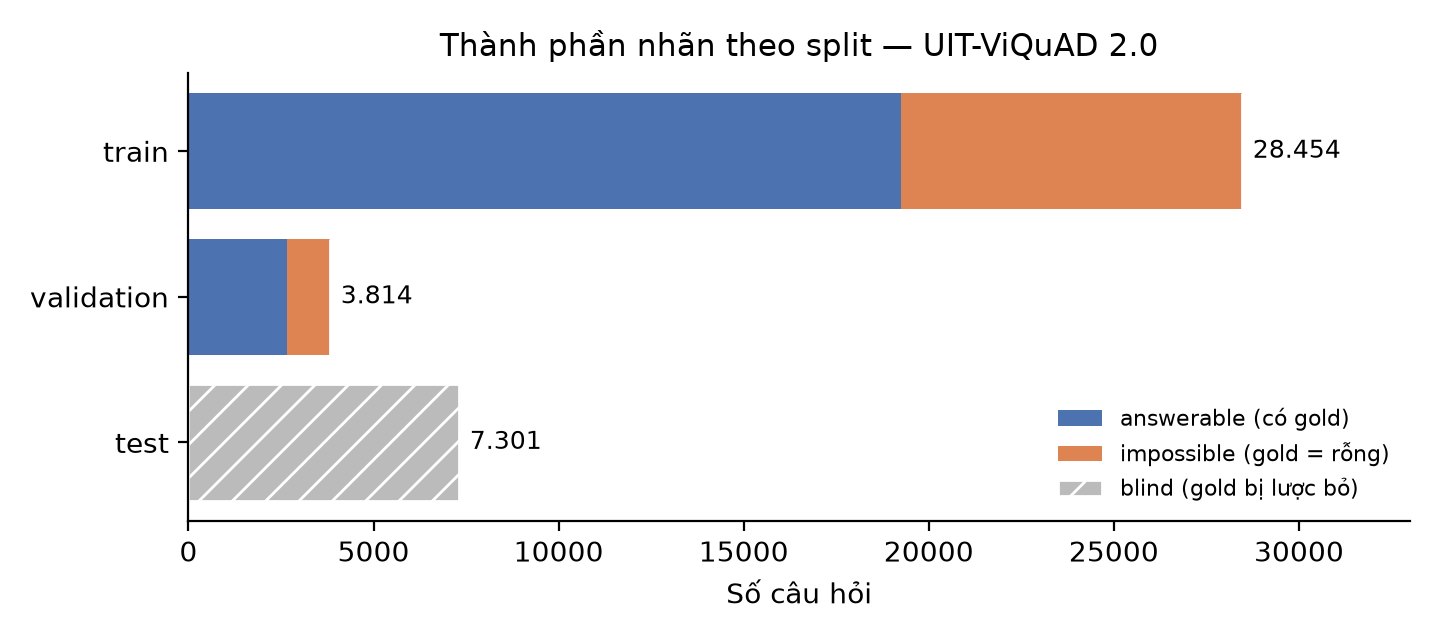
\includegraphics[width=0.78\textwidth]{figures/dataset_composition.png}
\caption{Thành phần nhãn theo split. Toàn bộ test split có đáp án bị lược bỏ nên không chấm được}
\label{fig:dataset-composition}
\end{figure}

\begin{figure}[htbp]
\centering
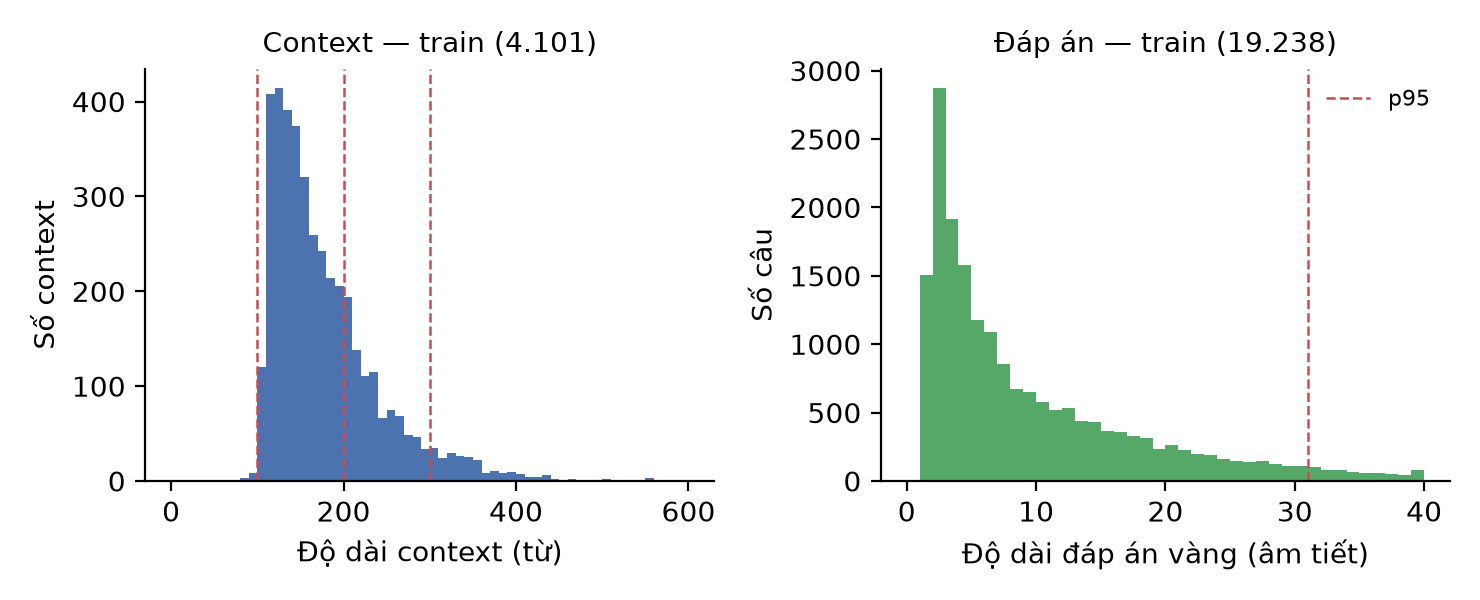
\includegraphics[width=0.88\textwidth]{figures/length_distributions.png}
\caption{Phân phối độ dài đoạn văn (trái; đường đứt là biên các nhóm 100/200/300 từ) và độ dài đáp án vàng (phải) trên tập train}
\label{fig:length-dist}
\end{figure}

\subsubsection{Test split là tập ẩn nhãn}
\label{sec:blind}

Kiểm tra trực tiếp cho thấy \textbf{cả 7.301 câu của test split đều có đáp án rỗng} đồng thời
\code{is\_impossible = False}. Hai điều này mâu thuẫn nếu coi là nhãn thật (câu không phải
``không có đáp án'' thì phải có đáp án), nên đây là \emph{giá trị giữ chỗ}: đáp án bị lược bỏ,
nhiều khả năng để dùng cho bảng xếp hạng của cuộc thi. Hệ quả:

\begin{enumerate}
  \item \textbf{Mọi kết quả trong báo cáo được đo trên validation split}, không phải test.
        Đây là tính chất của phiên bản dữ liệu công khai, không phải lựa chọn của nhóm.
  \item Validation đóng vai trò tập đánh giá cuối. Tập này \emph{có} được dùng để chọn epoch
        tốt nhất khi fine-tune (trên mẫu 300 câu), nên kết quả của hai mô hình fine-tune có
        thể lạc quan nhẹ so với một tập kiểm tra độc lập hoàn toàn (Mục~\ref{sec:limitations}).
  \item Test split còn chia sẻ 449 đoạn văn với train và 133 đoạn văn với validation. Điều
        này không ảnh hưởng đến kết quả của đồ án vì test không được chấm, nhưng là cảnh báo
        cho bất kỳ ai định dùng test split làm dữ liệu bổ sung hoặc tự gán nhãn lại.
\end{enumerate}

Train và validation không chia sẻ đoạn văn nào; \code{assert\_no\_leakage} xác nhận điều này
trước mỗi lần fine-tune (nhật ký huấn luyện: \emph{``4101 train ctx, 557 val ctx, giao nhau = 0''}).

\subsubsection{Phân bố từ để hỏi}

Để mô tả dữ liệu, câu hỏi validation được phân nhóm bằng từ khoá để hỏi
(Bảng~\ref{tab:wh}). Đây là phân nhóm từ khoá thô chỉ phục vụ mô tả, không dùng trong đánh giá.
Câu hỏi chứa ``gì'' và ``nào'' chiếm 57,9\%, phản ánh tính chất bách khoa của Wikipedia: phần
lớn câu hỏi yêu cầu một thực thể, khái niệm hoặc thuộc tính. Câu hỏi nguyên nhân (``vì sao'',
``tại sao'') chỉ chiếm 5,1\%.

\begin{table}[htbp]
\centering
\caption{Phân bố từ để hỏi trên validation (3.814 câu, phân nhóm theo từ khoá)}
\label{tab:wh}
\renewcommand{\arraystretch}{1.1}
\small
\begin{tabular}{@{}l r r @{\hspace{2.2em}} l r r@{}}
\toprule
\textbf{Từ khoá} & \textbf{Số câu} & \textbf{\%} & \textbf{Từ khoá} & \textbf{Số câu} & \textbf{\%} \\
\midrule
gì & 1.156 & 30,3 & vì sao & 115 & 3,0 \\
nào & 1.051 & 27,6 & khi nào & 93 & 2,4 \\
ai & 347 & 9,1 & năm nào & 84 & 2,2 \\
như thế nào & 315 & 8,3 & ở đâu & 80 & 2,1 \\
bao nhiêu & 301 & 7,9 & tại sao & 80 & 2,1 \\
không khớp từ khoá nào & 161 & 4,2 & mấy & 31 & 0,8 \\
\bottomrule
\end{tabular}
\end{table}

\subsection{Thiết lập thực nghiệm}
\label{sec:setup}

\begin{itemize}
  \item \textbf{Tập đánh giá.} Mẫu ngẫu nhiên $n = 500$ câu từ validation, lấy bằng
        \code{reproducible\_subset(seed=42)}, \emph{giống hệt nhau cho cả bốn mô hình}. Mẫu gồm 331
        đoạn văn; 139 câu không có đáp án (27,80\%) và 361 câu có đáp án. Theo nhóm độ dài
        đoạn văn: \code{<100}: 1, \code{100-200}: 405, \code{200-300}: 85, \code{300+}: 9. Theo
        loại câu hỏi (chỉ câu có đáp án): 143 \code{single-sentence}, 218 \code{multi-sentence}.
        Các con số này được đếm lại khi viết báo cáo và khớp với tệp kết quả, xác nhận mẫu tái
        lập được.
  \item \textbf{Vì sao 500 câu.} Mẫu con giữ vòng lặp thử nghiệm ngắn. Cái giá là độ bất định:
        với $n = 500$, nửa khoảng tin cậy 95\% của EM là khoảng $\pm 4$ điểm
        (công thức~\eqref{eq:ci}). Mọi so sánh bên dưới được diễn giải có tính đến độ bất định
        này. Harness hỗ trợ đánh giá toàn bộ 3.814 câu (\code{--full}); lần chạy đó chưa được
        thực hiện.
  \item \textbf{Suy luận.} \code{max\_length} $= 384$, \code{doc\_stride} $= 128$, ngưỡng
        $\tau = 0$; $L_{\max} = 30$ cho XLM-R và mBERT, $L_{\max} = 64$ cho ViSoBERT. Mỗi câu hỏi
        được xử lý riêng (batch size 1) để đo độ trễ.
  \item \textbf{Truy vết.} Bảng~\ref{tab:provenance} liệt kê commit và thời điểm sinh từng tệp
        kết quả. Hai commit khác nhau; giữa chúng, mã nguồn của các module đánh giá
        (\code{metrics}, \code{normalize}, \code{data}, \code{tagging}, \code{windowing},
        \code{transformer\_qa}, \code{baseline\_tfidf}, \code{evaluate}) \emph{không thay đổi} ---
        chỉ có script huấn luyện được tái cấu trúc và giá trị $L_{\max}$ mặc định của
        \code{run\_eval.py} được tách theo mô hình. Nhật ký chạy xác nhận giá trị $L_{\max}$ thực tế
        của từng mô hình.
\end{itemize}

\begin{table}[htbp]
\centering
\caption{Nguồn gốc các tệp kết quả (thời điểm theo UTC)}
\label{tab:provenance}
\renewcommand{\arraystretch}{1.12}
\small
\begin{tabular}{@{}l l l l l@{}}
\toprule
\textbf{Mô hình} & \textbf{Tệp kết quả} & \textbf{Commit} & \textbf{Thời điểm} & \textbf{Thiết bị} \\
\midrule
TF-IDF & \code{eval\_baseline\_validation.json} & \code{590e775} & 2026-09-12 14:06:43 & mps \\
XLM-R & \code{eval\_xlmr\_validation.json} & \code{c63b28c} & 2026-09-12 11:27:54 & mps \\
mBERT & \code{eval\_mbert\_validation.json} & \code{590e775} & 2026-09-12 14:03:03 & mps \\
ViSoBERT & \code{eval\_visobert\_validation.json} & \code{c63b28c} & 2026-09-12 11:28:13 & mps \\
\bottomrule
\end{tabular}
\end{table}

\subsection{Kết quả tổng thể}
\label{sec:overall}

Bảng~\ref{tab:main} là kết quả chính; Hình~\ref{fig:model-comparison} trực quan hoá EM và F1.
Nửa khoảng tin cậy 95\% của EM được ghi sau dấu $\pm$.

\begin{table}[htbp]
\centering
\caption{Kết quả chính trên validation, $n = 500$ (cùng mẫu cho mọi mô hình)}
\label{tab:main}
\renewcommand{\arraystretch}{1.2}
\small
\begin{tabular}{@{}l c c r r r@{}}
\toprule
\textbf{Mô hình} & \textbf{Loại} & \textbf{Fine-tune} & \textbf{EM} & \textbf{F1} & \textbf{F1 $-$ EM} \\
\midrule
TF-IDF & truy hồi câu & không & 0,80 $\pm$ 0,78 & 23,09 & 22,29 \\
ViSoBERT + QA & encoder tiếng Việt & có & 27,80 $\pm$ 3,93 & 31,31 & 3,51 \\
XLM-R squad2 & encoder đa ngữ & zero-shot & 40,60 $\pm$ 4,30 & 56,84 & 16,24 \\
\textbf{mBERT + QA} & encoder đa ngữ & có & \textbf{50,80 $\pm$ 4,38} & \textbf{59,49} & 8,69 \\
\bottomrule
\end{tabular}
\end{table}

\begin{figure}[htbp]
\centering
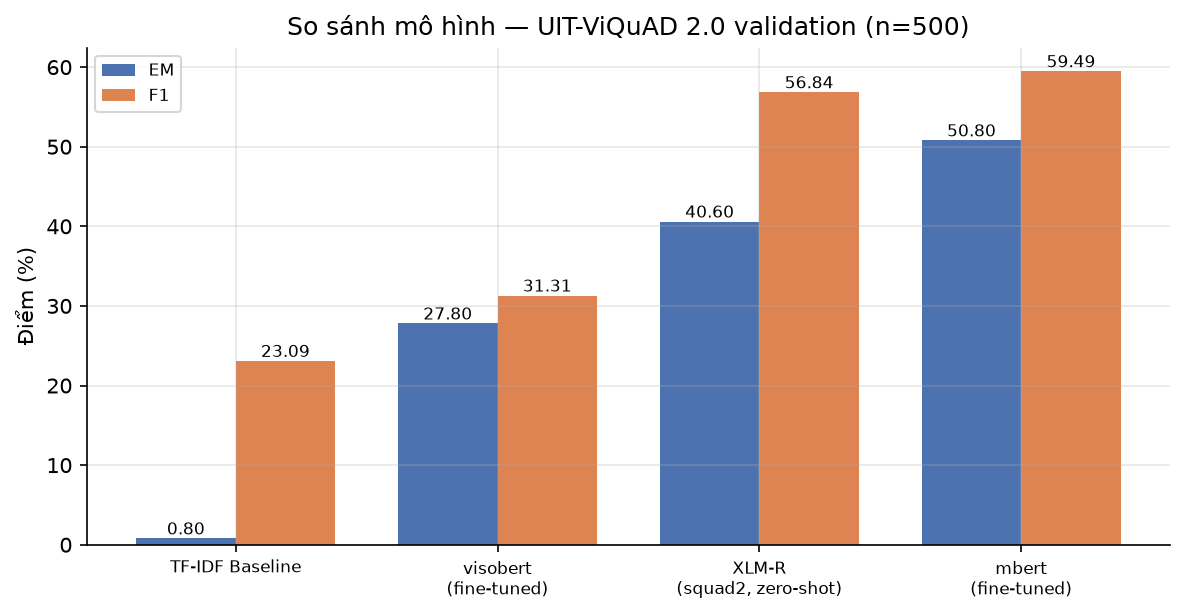
\includegraphics[width=0.8\textwidth]{figures/model_comparison.png}
\caption{EM và F1 của bốn mô hình trên cùng mẫu 500 câu validation}
\label{fig:model-comparison}
\end{figure}

Ba nhận xét chính:

\begin{enumerate}
  \item \textbf{Mọi mô hình Transformer đều vượt baseline, và mBERT fine-tune dẫn đầu cả hai
        metric.} Chênh lệch EM giữa mBERT và XLM-R là 10,20 điểm. Kiểm định chênh lệch hai tỉ
        lệ theo xấp xỉ chuẩn --- coi hai mẫu độc lập, một giả định thận trọng vì hai mô hình
        được chấm trên cùng câu hỏi --- cho nửa khoảng tin cậy 6,14 điểm ($z = 3{,}25$), nên chênh
        lệch EM này có ý nghĩa thống kê. Chênh lệch F1 (2,65 điểm) nhỏ hơn nhiều và cần phân
        tích tách nhóm ở mục sau để diễn giải.
  \item \textbf{Khoảng cách EM--F1 của baseline (22,29 điểm) khớp với cơ chế của nó.} TF-IDF
        trả về cả một câu, trong khi đáp án vàng có trung vị 6 âm tiết: câu trả về thường
        \emph{chứa} đáp án nên có overlap token (F1), nhưng gần như không bao giờ \emph{trùng
        khít} (chỉ 4 trên 361 câu có đáp án đạt EM). Đây là minh hoạ trực quan rằng EM và F1
        đo hai thứ khác nhau. EM của baseline trên câu không có đáp án bằng 0 vì nó luôn trả
        về một câu.
  \item \textbf{ViSoBERT đứng sau XLM-R zero-shot dù đã fine-tune} --- đúng tín hiệu báo động
        ``mô hình fine-tune kém hơn zero-shot'' đã định nghĩa trước. Khoảng cách EM--F1 rất nhỏ
        (3,51) là manh mối đầu tiên: mô hình hiếm khi cho điểm bán phần. Nguyên nhân được điều
        tra ở Mục~\ref{sec:visobert-analysis}.
\end{enumerate}

\subsection{Tách theo câu có đáp án và câu không có đáp án}
\label{sec:ans-imp}

Vì EM tổng trộn hai kỹ năng (Mục~\ref{sec:metrics-theory}), Bảng~\ref{tab:ans-imp} và
Hình~\ref{fig:ans-imp} tách kết quả theo hai nhóm câu.

\begin{table}[htbp]
\centering
\caption{Kết quả tách theo nhóm câu hỏi (validation, $n = 500$)}
\label{tab:ans-imp}
\renewcommand{\arraystretch}{1.2}
\small
\begin{tabular}{@{}l r r r r r@{}}
\toprule
& \multicolumn{3}{c}{\textbf{Câu có đáp án} ($n = 361$)} & \multicolumn{2}{c}{\textbf{Không có đáp án} ($n = 139$)} \\
\cmidrule(lr){2-4}\cmidrule(l){5-6}
\textbf{Mô hình} & \textbf{EM} & \textbf{F1} & \textbf{Số câu đúng} & \textbf{EM} & \textbf{Số câu đúng} \\
\midrule
TF-IDF & 1,11 $\pm$ 1,08 & 31,99 & 4 & 0,00 & 0 \\
ViSoBERT & 6,93 $\pm$ 2,62 & 11,78 & 25 & \textbf{82,01 $\pm$ 6,38} & 114 \\
XLM-R & 45,71 $\pm$ 5,14 & \textbf{68,20} & 165 & 27,34 $\pm$ 7,41 & 38 \\
mBERT & \textbf{54,57 $\pm$ 5,14} & 66,60 & 197 & 41,01 $\pm$ 8,18 & 57 \\
\bottomrule
\end{tabular}
\par\vspace{2pt}
{\footnotesize Trên câu không có đáp án, F1 luôn bằng EM nên không ghi riêng. ``Số câu đúng'' là số câu đạt EM $= 1$, suy ra từ EM và $n$.}
\end{table}

\begin{figure}[htbp]
\centering
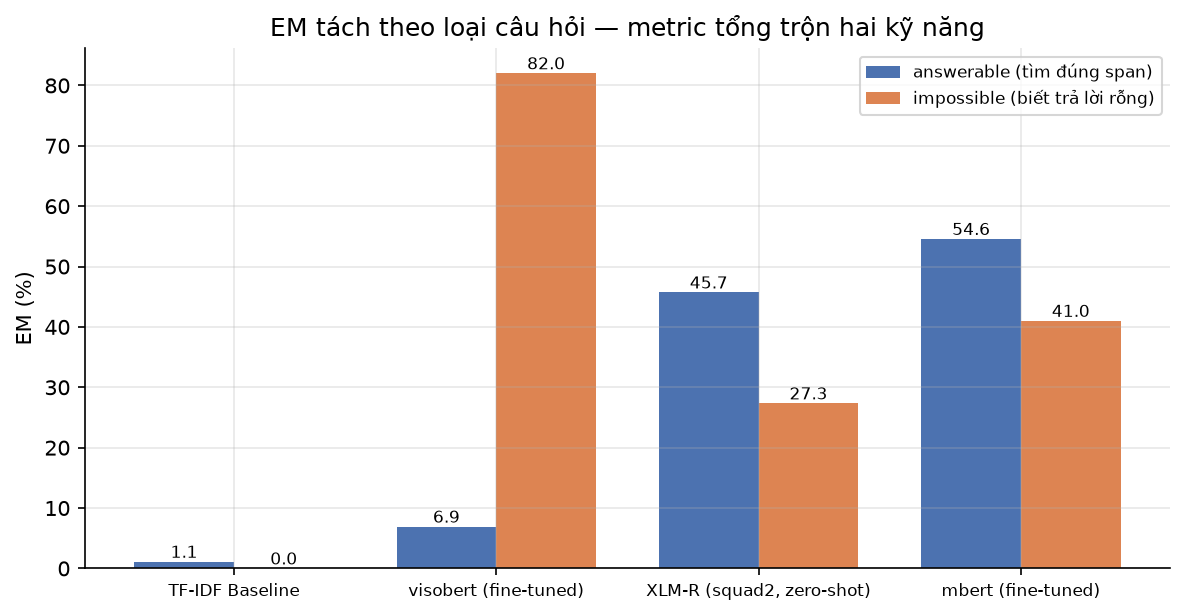
\includegraphics[width=0.8\textwidth]{figures/em_answerable_vs_impossible.png}
\caption{EM tách theo câu có đáp án (tìm đúng span) và câu không có đáp án (biết trả lời rỗng)}
\label{fig:ans-imp}
\end{figure}

\subsubsection{mBERT so với XLM-R: hai kỹ năng, hai câu chuyện}

Vì điểm tổng là trung bình có trọng số của hai nhóm, có thể phân rã chính xác chênh lệch
giữa mBERT và XLM-R thành phần đóng góp của từng nhóm, với trọng số $361/500$ và $139/500$
(Bảng~\ref{tab:decomp}).

\begin{table}[htbp]
\centering
\caption{Phân rã chênh lệch mBERT $-$ XLM-R theo nhóm câu hỏi (đơn vị: điểm)}
\label{tab:decomp}
\renewcommand{\arraystretch}{1.2}
\small
\begin{tabular}{@{}l r r r@{}}
\toprule
\textbf{Metric} & \textbf{Từ câu có đáp án} & \textbf{Từ câu không có đáp án} & \textbf{Tổng chênh lệch} \\
\midrule
EM & $+6{,}40$ & $+3{,}80$ & $+10{,}20$ \\
F1 & $-1{,}15$ & $+3{,}80$ & $+2{,}65$ \\
\bottomrule
\end{tabular}
\end{table}

Bảng~\ref{tab:decomp} cho hai kết luận khác nhau tuỳ metric --- và cả hai đều đúng:

\begin{itemize}
  \item \textbf{Trên F1}, toàn bộ lợi thế của mBERT đến từ câu không có đáp án. Trên câu có đáp
        án, XLM-R có F1 cao hơn 1,60 điểm; chênh lệch này nhỏ so với độ bất định ở $n = 361$,
        nên \emph{không đủ bằng chứng} để nói mô hình nào tìm vùng đáp án tốt hơn.
  \item \textbf{Trên EM}, phần lớn lợi thế (6,40 trên 10,20 điểm) đến từ câu \emph{có} đáp án:
        mBERT trùng khít đáp án vàng ở 197 câu so với 165 câu của XLM-R (chênh 8,86 điểm; nửa
        khoảng tin cậy của chênh lệch 7,27; $z = 2{,}39$).
\end{itemize}

Kết hợp lại: \emph{XLM-R zero-shot tìm được vùng chứa đáp án tốt ngang mBERT, nhưng chọn ranh
giới đáp án khác với quy ước gán nhãn của UIT-ViQuAD}. Khoảng cách F1--EM trên câu có đáp án
của XLM-R là 22,50 điểm, gần gấp đôi mBERT (12,03). Các dự đoán mẫu minh hoạ điều này
(Bảng~\ref{tab:qualitative}): với câu hỏi về số người Việt ở Montréal, XLM-R trả lời ``100''
trong khi đáp án vàng là ``100 người''. Fine-tune trên dữ liệu trong miền dạy mô hình quy ước
ranh giới này --- lợi ích mà chuyển giao zero-shot không mang lại. Kỹ năng thứ hai, \emph{từ
chối}, cũng được cải thiện: EM trên câu không có đáp án tăng từ 27,34 lên 41,01 (chênh 13,67;
nửa khoảng tin cậy 11,03; $z = 2{,}43$). Tuy vậy, cả hai mô hình vẫn trả lời nhầm phần lớn câu
không có đáp án --- mBERT chỉ từ chối đúng 57 trên 139 câu.

\subsubsection{ViSoBERT: điểm tổng đến từ việc từ chối}

EM tổng của ViSoBERT (27,80) \textbf{bằng đúng tỉ lệ câu không có đáp án của mẫu} (27,80\%).
Tách nhóm cho thấy lý do: mô hình từ chối đúng 114 trên 139 câu không có đáp án (EM 82,01)
nhưng chỉ trả lời trùng khít 25 trên 361 câu có đáp án (EM 6,93). Gần như toàn bộ điểm của
ViSoBERT đến từ hành vi trả về chuỗi rỗng. Script \code{check\_hypotheses.py} phát hiện tự động
hiện tượng này bằng tín hiệu báo động \code{score\_equals\_impossible\_rate}. Nếu chỉ nhìn điểm
tổng, ViSoBERT trông như ``kém hơn XLM-R 13 điểm''; thực tế nó gần như không thực hiện được tác
vụ tìm đáp án.

\subsection{Phân tích theo loại câu hỏi}
\label{sec:by-qtype}

Bảng~\ref{tab:qtype} và Hình~\ref{fig:qtype} so sánh kết quả trên câu hỏi cần bằng chứng từ
một câu (\code{single-sentence}) và từ nhiều câu (\code{multi-sentence}), theo heuristic ở
Mục~\ref{sec:tagging}. Tổng của bảng là 361, không phải 500, vì chỉ câu có đáp án được phân loại.

\begin{table}[htbp]
\centering
\caption{Kết quả theo phạm vi suy luận của câu hỏi (chỉ câu có đáp án; nhãn do heuristic gán)}
\label{tab:qtype}
\renewcommand{\arraystretch}{1.2}
\small
\begin{tabular}{@{}l r r r r r@{}}
\toprule
& \multicolumn{2}{c}{\textbf{single-sentence} ($n = 143$)} & \multicolumn{2}{c}{\textbf{multi-sentence} ($n = 218$)} & \\
\cmidrule(lr){2-3}\cmidrule(lr){4-5}
\textbf{Mô hình} & \textbf{EM} & \textbf{F1} & \textbf{EM} & \textbf{F1} & \textbf{Chênh F1} \\
\midrule
TF-IDF & 1,40 & 35,87 & 0,92 & 29,44 & 6,44 \\
ViSoBERT & 11,19 & 17,82 & 4,13 & 7,82 & 10,00 \\
XLM-R & 50,35 & 70,92 & 42,66 & \textbf{66,42} & 4,51 \\
mBERT & \textbf{60,84} & \textbf{73,51} & \textbf{50,46} & 62,07 & 11,44 \\
\bottomrule
\end{tabular}
\end{table}

\begin{figure}[htbp]
\centering
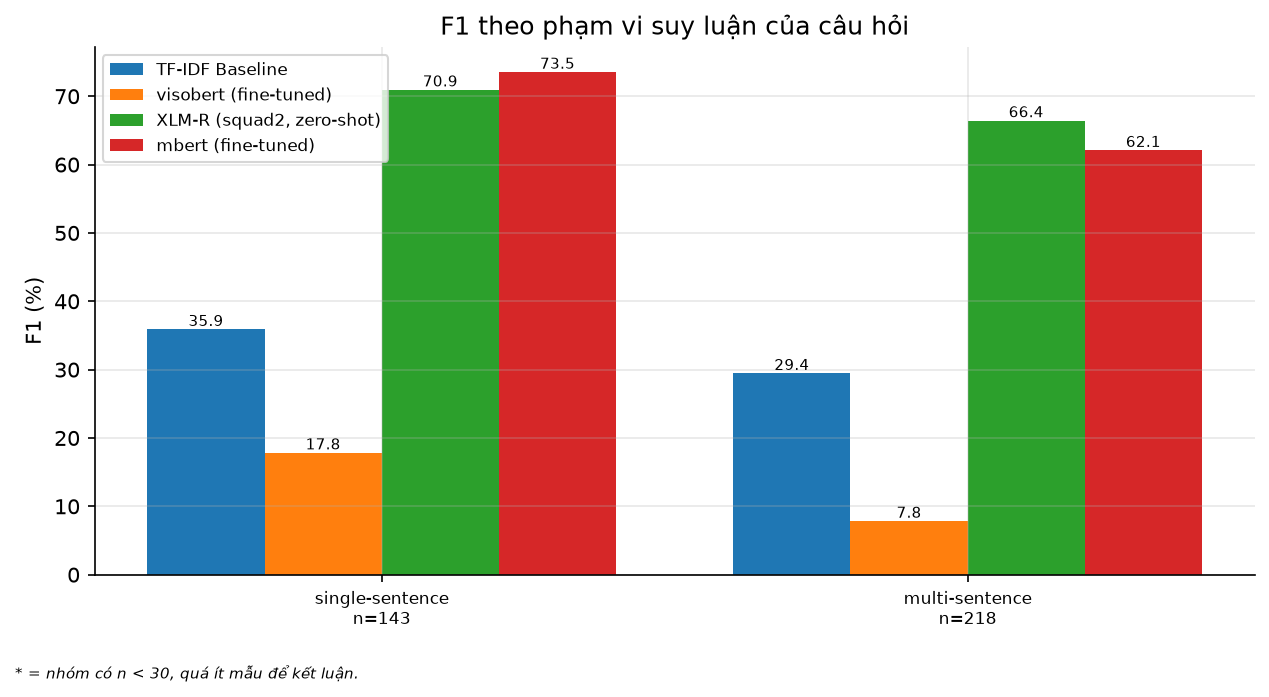
\includegraphics[width=0.8\textwidth]{figures/f1_by_question_type.png}
\caption{F1 theo phạm vi suy luận của câu hỏi}
\label{fig:qtype}
\end{figure}

\textbf{Xu hướng nhất quán:} cả bốn mô hình đều có F1 thấp hơn trên nhóm \code{multi-sentence},
với mức chênh từ 4,51 (XLM-R) đến 11,44 điểm (mBERT). \textbf{Bằng chứng thống kê ở mức vừa
phải:} với mBERT, chênh lệch EM giữa hai nhóm là 10,38 điểm trong khi nửa khoảng tin cậy của
chênh lệch là 10,39 --- nằm đúng tại ngưỡng ý nghĩa; với XLM-R, chênh lệch EM (7,69) nhỏ hơn
nửa khoảng tin cậy (10,50). Hai nhóm chỉ có 143 và 218 câu.

Một quan sát đáng chú ý: trên nhóm \code{multi-sentence}, XLM-R zero-shot có F1 cao hơn mBERT
(66,42 so với 62,07), trong khi mBERT dẫn rõ trên \code{single-sentence}. Một cách giải thích
hợp lý là fine-tune giúp mBERT khai thác tốt câu hỏi trùng từ vựng cao với một câu trong đoạn
văn, còn XLM-R --- tiền huấn luyện trên lượng dữ liệu lớn hơn nhiều --- bền vững hơn khi câu hỏi
diễn đạt khác đoạn văn. Đây là \emph{giả thuyết} chưa được kiểm chứng: với cỡ nhóm hiện tại,
chênh lệch 4,35 điểm F1 chưa đủ để kết luận.

\begin{warnbox}
\textbf{Diễn giải có giới hạn.} Heuristic \code{question\_type} dựa trên độ trùng từ vựng giữa
câu hỏi và một câu của đoạn văn. Vì vậy nhóm \code{multi-sentence} vừa gồm câu hỏi thực sự cần
suy luận nhiều câu, vừa gồm câu hỏi đơn giản nhưng \emph{được diễn đạt lại}. Kết quả trên cho
thấy các mô hình kém hơn trên câu hỏi \emph{ít trùng từ với một câu đơn lẻ}; nó không tách được
riêng ảnh hưởng của suy luận nhiều câu.
\end{warnbox}

\subsection{Phân tích theo độ dài đoạn văn}
\label{sec:by-length}

\begin{table}[htbp]
\centering
\caption{F1 theo độ dài đoạn văn (số từ); nhóm có $n < 30$ được đánh dấu $^\dagger$ và không dùng để kết luận}
\label{tab:length}
\renewcommand{\arraystretch}{1.2}
\small
\begin{tabular}{@{}l r r r r@{}}
\toprule
\textbf{Mô hình} & \textbf{<100}$^\dagger$ & \textbf{100--200} & \textbf{200--300} & \textbf{300+}$^\dagger$ \\
 & $n=1$ & $n=405$ & $n=85$ & $n=9$ \\
\midrule
TF-IDF & 66,67 & 23,50 & 21,27 & 17,26 \\
ViSoBERT & 0,00 & 30,76 & 33,58 & 37,78 \\
XLM-R & 88,89 & 58,15 & 50,06 & 58,78 \\
mBERT & 33,33 & 59,16 & 62,97 & 44,44 \\
\midrule
\bottomrule
\end{tabular}
\par\vspace{2pt}
{\footnotesize EM của nhóm 100--200 / 200--300: TF-IDF 0,99 / 0,00; ViSoBERT 26,91 / 31,76; XLM-R 41,48 / 37,65; mBERT 50,62 / 52,94.}
\end{table}

\begin{figure}[htbp]
\centering
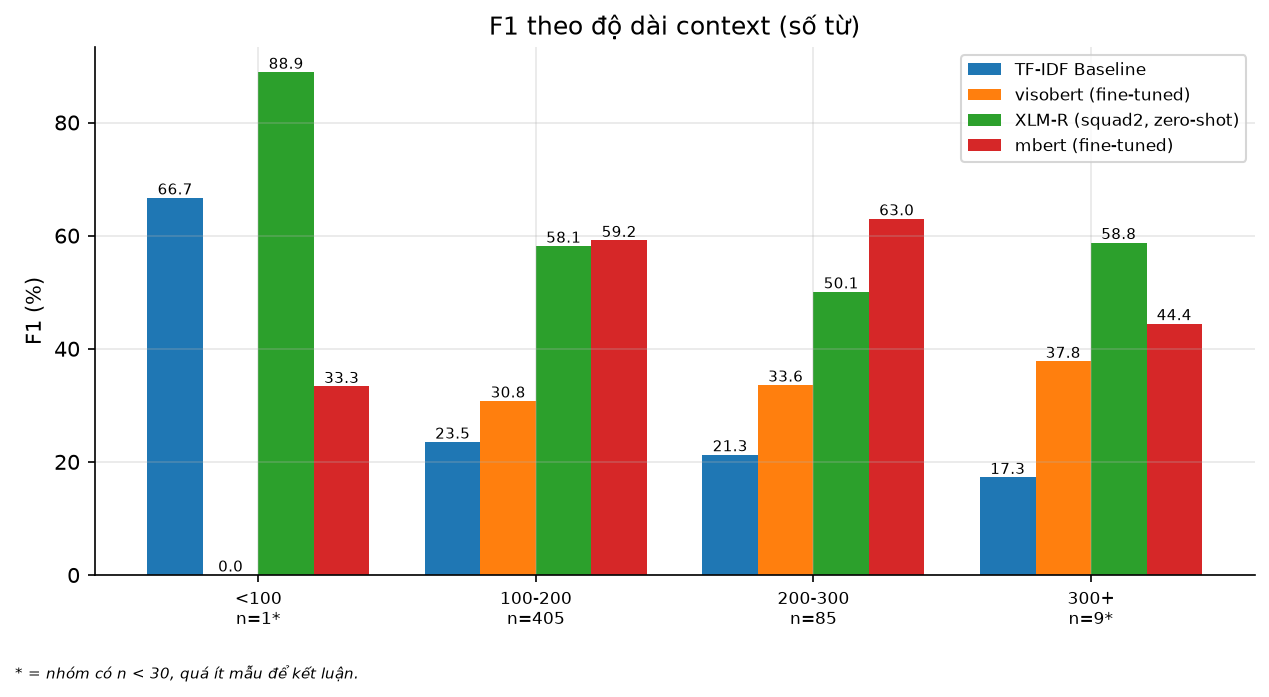
\includegraphics[width=0.8\textwidth]{figures/f1_by_context_length.png}
\caption{F1 theo độ dài đoạn văn. Dấu * đánh dấu nhóm có $n < 30$}
\label{fig:length}
\end{figure}

Bảng~\ref{tab:length} và Hình~\ref{fig:length} cho thấy \textbf{không có xu hướng nhất quán}
theo độ dài đoạn văn trong phạm vi dữ liệu có đủ mẫu. Chỉ hai nhóm \code{100-200} ($n = 405$) và
\code{200-300} ($n = 85$) đủ lớn để so sánh; giữa hai nhóm này, F1 của TF-IDF và XLM-R giảm (lần
lượt $-2{,}23$ và $-8{,}09$ điểm) còn F1 của mBERT và ViSoBERT tăng ($+3{,}82$ và $+2{,}82$). Với
$n = 85$, không chênh lệch nào trong số này đủ lớn để loại trừ biến động ngẫu nhiên. Hai nhóm
\code{<100} ($n = 1$) và \code{300+} ($n = 9$) bị gắn cờ \code{unreliable}: với $n = 1$, một câu
đúng hay sai làm điểm nhóm dao động 100 điểm.

Kết quả này nhất quán với cấu hình: ở \code{max\_length} $= 384$, chỉ 16 trên 557 đoạn văn
validation dài hơn 357 token theo tokenizer của mBERT, nên cơ chế cửa sổ trượt --- nơi đáp án có
thể rơi vào cửa sổ thiếu ngữ cảnh --- hiếm khi được kích hoạt. Mẫu 500 câu chứa quá ít đoạn văn
dài để đo ảnh hưởng của cơ chế này; câu hỏi ``độ dài đoạn văn ảnh hưởng thế nào'' vì vậy
\emph{chưa được trả lời} bởi thực nghiệm hiện tại (xem hướng phát triển).

\subsection{Quá trình huấn luyện}
\label{sec:curves}

\begin{table}[htbp]
\centering
\caption{Đường cong huấn luyện (validation: 300 câu ngẫu nhiên, seed 42)}
\label{tab:curves}
\renewcommand{\arraystretch}{1.18}
\footnotesize
\setlength{\tabcolsep}{5pt}
\begin{tabular}{@{}l c r r r r r@{}}
\toprule
\textbf{Mô hình} & \textbf{Epoch} & \textbf{Loss train} & \textbf{Val EM} & \textbf{Val F1} & \textbf{F1 $-$ EM} & \textbf{Thời gian (s)} \\
\midrule
mBERT ($\eta = 3\cdot10^{-5}$) & 1 & 2,1316 & 46,00 & 58,39 & 12,39 & 2.066 \\
 & 2 & 1,2960 & 52,00 & \textbf{59,75} & 7,75 & 2.100 \\
\midrule
ViSoBERT ($\eta = 5\cdot10^{-5}$) & 1 & 3,0512 & 25,67 & 25,67 & \textcolor{badred}{0,00} & 2.417 \\
 & 2 & 2,5678 & 25,33 & 25,61 & \textcolor{badred}{0,28} & 2.475 \\
 & 3 & 2,1908 & 27,00 & \textbf{30,48} & 3,48 & 6.798$^\ddagger$ \\
\bottomrule
\end{tabular}
\par\vspace{2pt}
{\footnotesize $^\ddagger$ Thời gian epoch 3 bị nhiễu do một tác vụ chẩn đoán chạy song song tranh GPU; không dùng làm số đo hiệu năng. Epoch tốt nhất (in đậm) được chọn làm mô hình cuối.}
\end{table}

\begin{figure}[htbp]
\centering
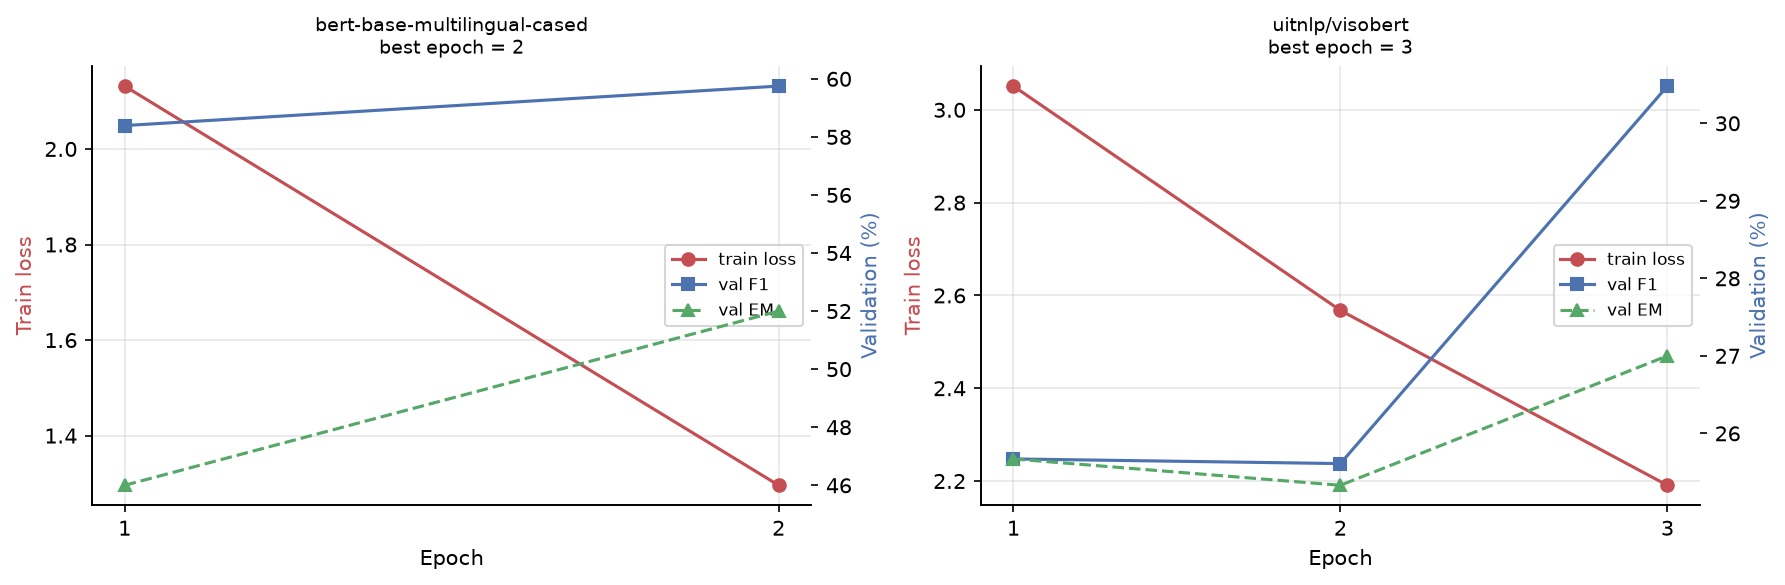
\includegraphics[width=0.95\textwidth]{figures/training_curves.png}
\caption{Đường cong huấn luyện: loss train (trục trái) và EM/F1 validation (trục phải) của mBERT (trái) và ViSoBERT (phải)}
\label{fig:curves}
\end{figure}

\paragraph{mBERT.} Loss train giảm mạnh từ 2,1316 xuống 1,2960 và F1 validation tăng ở epoch 2,
nên hàm chẩn đoán kết luận \code{still\_improving}: \emph{chưa có dấu hiệu overfitting}, và có
thể còn thiếu epoch. Cần thận trọng với kết luận ``còn cải thiện'': mức tăng F1 (1,36 điểm) nhỏ
so với độ bất định của mẫu 300 câu; mức tăng EM (6,00 điểm) rõ hơn. Một thí nghiệm với 3--4
epoch là cần thiết để xác định điểm dừng tối ưu. Kết quả epoch 2 trên mẫu 300 câu (EM 52,00) nhất
quán với kết quả trên mẫu 500 câu (EM 50,80), vì hai mẫu được lấy bằng cùng hàm và cùng seed.

\paragraph{ViSoBERT.} Ở epoch 1 và 2, EM và F1 validation gần như bằng nhau (chênh 0,00 và 0,28)
và cùng xấp xỉ tỉ lệ câu không có đáp án của mẫu 300 câu (25,67\%). Theo phân tích ở
Mục~\ref{sec:metrics-theory}, đây là dấu hiệu mô hình \emph{suy sụp về hành vi luôn trả rỗng}:
câu không có đáp án được 1 điểm, câu có đáp án được 0 điểm, không có điểm bán phần. Ở epoch 3,
F1 tách khỏi EM (chênh 3,48), cho thấy mô hình bắt đầu thoát khỏi trạng thái suy sụp, nhưng vẫn
kém xa mBERT. Loss train vẫn giảm đều (3,05 $\to$ 2,19) --- minh hoạ rằng loss giảm không đảm
bảo mô hình học đúng tác vụ.

\subsection{Điều tra nguyên nhân thất bại của ViSoBERT}
\label{sec:visobert-analysis}

Một mô hình được fine-tune mà kém hơn mô hình zero-shot là tín hiệu báo động được định nghĩa
trước, nên nhóm điều tra theo phương pháp loại trừ: lần lượt kiểm tra các nguyên nhân do
\emph{cấu hình} trước khi quy cho \emph{mô hình}.

\subsubsection{Loại trừ các nguyên nhân cấu hình}

Bảng~\ref{tab:confounds} tóm tắt quá trình. Các phép đo trong bảng đến từ những lần chạy chẩn
đoán được ghi lại trong nhật ký commit của dự án (\code{abb6d8f}, \code{c63b28c}, \code{388b0ba}),
không được lưu thành tệp \code{results/*.json} riêng; chúng có mức truy vết thấp hơn kết quả chính.

\begin{table}[htbp]
\centering
\caption{Quá trình loại trừ nguyên nhân cấu hình cho ViSoBERT}
\label{tab:confounds}
\renewcommand{\arraystretch}{1.22}
\small
\begin{tabularx}{\textwidth}{@{}>{\raggedright\arraybackslash}p{3.3cm} >{\raggedright\arraybackslash}p{3.6cm} L@{}}
\toprule
\textbf{Nghi vấn} & \textbf{Kiểm tra} & \textbf{Kết quả} \\
\midrule
Số vị trí tối đa nhỏ hơn \code{max\_length} & Đọc cấu hình mô hình & \code{max\_position\_embeddings} $= 514$ --- không phải nguyên nhân \\
$L_{\max} = 30$ token quá ngắn với tokenizer 15k & Đo độ dài token của đáp án vàng trên 4.000 mẫu train & \textbf{Là nguyên nhân thật}: 25,2\% đáp án vượt 30 token (mBERT: 10,8\%), p95 $= 64$ (mBERT: 40). Một phần tư đáp án \emph{không thể biểu diễn} được ở $L_{\max} = 30$. Sửa thành 64$^\ast$ \\
Tốc độ học quá thấp & Chạy lại với $\eta = 5\cdot10^{-5}$ \emph{và} $L_{\max} = 64$, 3 epoch & F1 validation từ 12,25 (lần chạy đầu, epoch 1) lên 30,48 (epoch 3): cải thiện nhưng vẫn kém xa mBERT (58,39 ngay epoch 1). Hai thay đổi cùng lúc nên không tách được đóng góp riêng của tốc độ học \\
Ngưỡng không trả lời $\tau$ lệch & Quét $\tau$ trên checkpoint epoch 2, 200 câu validation (31,5\% không có đáp án) & Bảng~\ref{tab:threshold}: giảm $\tau$ làm giảm tỉ lệ trả rỗng nhưng F1 tốt nhất chỉ 34,77; ép luôn trả lời thì EM còn 11,50 \\
\bottomrule
\end{tabularx}
\par\vspace{2pt}
{\footnotesize $^\ast$ Khi viết báo cáo, nhóm đo lại trên 2.698 đáp án vàng thuộc 4.000 câu đầu của tập train: p95 là 42 (mBERT) và 67 (ViSoBERT); tỉ lệ vượt 30 token là 12,0\% và 27,8\%. Cỡ mẫu khác lần đo gốc nhưng kết luận không đổi.}
\end{table}

\begin{table}[htbp]
\centering
\caption{Quét ngưỡng không trả lời $\tau$ cho ViSoBERT (checkpoint epoch 2, 200 câu validation)}
\label{tab:threshold}
\renewcommand{\arraystretch}{1.15}
\small
\begin{tabular}{@{}r r r r l@{}}
\toprule
$\tau$ & \textbf{EM} & \textbf{F1} & \textbf{\% dự đoán rỗng} & \textbf{Nhận xét} \\
\midrule
0,0 & 31,00 & 31,00 & 95\% & EM $=$ F1 $\approx$ tỉ lệ không có đáp án: suy sụp \\
$-2{,}0$ & 30,50 & 34,77 & 70\% & F1 tốt nhất trong các ngưỡng thử \\
$-10{,}0$ & 11,50 & 24,48 & 0\% & Ép luôn trả lời \\
\bottomrule
\end{tabular}
\end{table}

Khi bị ép trả lời mọi câu, ViSoBERT chỉ đạt EM 11,50: vấn đề không nằm ở ngưỡng quyết định mà ở
chỗ mô hình \emph{không định vị được đáp án}. Lần chạy đầu tiên ($L_{\max} = 30$,
$\eta = 3\cdot10^{-5}$) còn cho thấy một dạng suy thoái khác: 52\% dự đoán rỗng (trong khi chỉ
khoảng 25\% câu thực sự không có đáp án), phần còn lại lặp lại đúng một token ``ông''.

\subsubsection{Bằng chứng về mức độ phân mảnh token}

Sau khi loại trừ các nguyên nhân cấu hình đã kiểm tra, khác biệt đáng chú ý nhất giữa hai mô hình
là cách tokenizer biểu diễn văn bản Wikipedia tiếng Việt. Bảng~\ref{tab:tokenization} tổng hợp
các phép đo, thực hiện lại khi viết báo cáo bằng tokenizer lưu cùng checkpoint.

\begin{table}[htbp]
\centering
\caption{So sánh mức độ phân mảnh của hai tokenizer trên dữ liệu ViQuAD}
\label{tab:tokenization}
\renewcommand{\arraystretch}{1.18}
\small
\begin{tabularx}{\textwidth}{@{}L r r@{}}
\toprule
\textbf{Chỉ số} & \textbf{mBERT} & \textbf{ViSoBERT} \\
\midrule
Kích thước ma trận nhúng (\code{vocab\_size} trong \code{config.json}) & 119.547 & 15.004 \\
Kích thước từ vựng thực tế (\code{len(tokenizer)}) & 119.547 & 15.002 \\
Số token của câu ``Hà Nội là thủ đô của nước Cộng hoà Xã hội chủ nghĩa Việt Nam.'' & 17 & 23 \\
Số token trung bình mỗi từ (557 đoạn văn validation) & 1,22 & 1,95 \\
Số token trung bình mỗi đoạn văn validation & 204,6 & 326,5 \\
Số đoạn văn validation dài hơn 357 token & 16 & 154 \\
Số cửa sổ huấn luyện sinh từ 28.454 câu train & 30.540 & 40.984 \\
Độ trễ suy luận trung bình (ms/câu) & 12,26 & 22,73 \\
\bottomrule
\end{tabularx}
\end{table}

\noindent Tokenizer của ViSoBERT tách câu ví dụ thành
\code{▁Hà ▁N ội ▁là ▁thủ ▁đô ▁c ủa ▁n ước ▁C ộng} \dots{}, trong khi mBERT giữ nguyên
\code{Hà Nội là thủ đô của nước Cộng} \dots{}. Những từ rất phổ biến như ``của'', ``nước'' bị cắt
đôi, cho thấy từ vựng 15.002 token của ViSoBERT không bao phủ tốt văn phong Wikipedia.
Hai dòng đầu của Bảng~\ref{tab:tokenization} chênh nhau đúng 2: \code{config.json} khai
báo ma trận nhúng 15.004 hàng trong khi tokenizer chỉ sinh ra 15.002 token phân biệt,
nghĩa là có hai hàng nhúng không token nào ánh xạ tới. Chi tiết này không ảnh hưởng kết
quả, nhưng được ghi lại vì hai con số rất dễ bị dùng lẫn cho nhau --- ``kích thước từ
vựng'' trong mọi lập luận của báo cáo này luôn là 15.002. Hệ quả
dây chuyền phù hợp với các quan sát: đoạn văn dài hơn khoảng 1,6 lần tính theo token, số đoạn văn
dài hơn 357 token tăng gần 10 lần, số cửa sổ huấn luyện tăng 34\%, độ trễ tăng gần gấp đôi dù mô
hình có ít tham số hơn (97,0 so với 177,3 triệu), và ranh giới đáp án phải được xác định trên các
mảnh token nhỏ hơn.

\subsubsection{Bốn yếu tố đủ để giải thích sự suy sụp}
\label{sec:visobert-factors}

Khi rà soát lại toàn bộ bằng chứng để viết báo cáo, nhóm nhận ra rằng \textbf{bốn yếu tố dưới đây
đã đủ để giải thích sự suy sụp mà không cần viện tới chất lượng của ViSoBERT như một encoder}.
Đây là điều chỉnh quan trọng so với cách trình bày ban đầu: một trong bốn yếu tố là \emph{nguyên
nhân cấu hình chưa được bù trừ}, chứ không phải nguyên nhân đã bị loại trừ.

\begin{enumerate}
  \item \textbf{Ngân sách cửa sổ chưa được bù trừ --- yếu tố mạnh nhất.} Cả hai mô hình dùng chung
        \code{max\_length} $= 384$ và \code{doc\_stride} $= 128$. Nhưng theo
        Bảng~\ref{tab:tokenization}, chỉ 16 trên 557 đoạn văn validation (2,9\%) vượt 357 token với
        tokenizer của mBERT, trong khi con số đó với ViSoBERT là 154 trên 557 (\textbf{27,6\%}) ---
        gấp gần mười lần. Mỗi cửa sổ thêm vào là một cơ hội nữa để điểm ``không trả lời'' thắng, và
        một khả năng nữa để span đáp án rơi vào cửa sổ thiếu ngữ cảnh. Tham số này được đặt theo
        cách tokenize của mBERT và \textbf{không được điều chỉnh lại cho ViSoBERT}.
  \item \textbf{Hàm mất mát chưa hội tụ.} Theo Bảng~\ref{tab:curves}, ViSoBERT kết thúc 3 epoch ở
        loss train 2,19, trong khi mBERT kết thúc chỉ 2 epoch ở 1,30. ViSoBERT được huấn luyện
        \emph{lâu hơn} mà vẫn dừng ở mức lỗi cao hơn rõ rệt.
  \item \textbf{Sức chứa mô hình.} 97,0 triệu tham số so với 177,3 triệu của mBERT --- nhỏ hơn
        khoảng 45\% (Bảng~\ref{tab:cost}).
  \item \textbf{Mất cân bằng lớp tạo ra một cực tiểu địa phương rất hấp dẫn.} Tập huấn luyện có
        32,39\% câu không có đáp án, nên chiến lược ``luôn trả rỗng'' đạt ngay khoảng 32\% độ chính
        xác mà không cần học gì. Với tốc độ học cao hơn ($5\cdot10^{-5}$ so với $3\cdot10^{-5}$ của
        mBERT), mô hình rơi vào hố này ngay epoch 1 và phải tới epoch 3 mới bắt đầu leo ra ---
        đúng hình dạng của đường cong trong Bảng~\ref{tab:curves}.
\end{enumerate}

\begin{warnbox}
\textbf{Cần nói rõ cho công bằng: trục \emph{độ dài đáp án} đã được bù trừ, trục \emph{độ dài
cửa sổ} thì chưa.} Nhóm \emph{đã} bù trừ $L_{\max}$ cho ViSoBERT --- \code{src/evaluation/cli.py}
đặt $L_{\max} = 64$ thay cho mặc định 30, chính vì tokenizer 15.002 token sinh ra đáp án dài hơn
tính theo token (Bảng~\ref{tab:confounds}). Nên độ dài đáp án \textbf{không} còn là nguyên nhân
của kết quả cuối cùng. Trục chưa được bù là \code{max\_length}, không phải
\code{max\_answer\_len}. Hai tham số này rất dễ bị nói lẫn, và sự khác biệt quyết định cách đọc
toàn bộ mục này.
\end{warnbox}

\begin{keybox}
\textbf{Kết luận và mức độ chắc chắn.} Trong thiết lập của đồ án, ViSoBERT kém mBERT rất xa trên
MRC Wikipedia tiếng Việt. Nhưng \textbf{bốn yếu tố ở Mục~\ref{sec:visobert-factors} --- trong đó
có một nguyên nhân cấu hình chưa được bù trừ --- đã đủ để giải thích khoảng cách này}, nên
\emph{không} rút ra được từ dữ liệu hiện có kết luận rằng tiền huấn luyện tiếng Việt không mang
lại lợi ích. Cách giải thích mà nhóm cho là hợp lý nhất --- \emph{từ vựng nhỏ phân mảnh mạnh văn
bản của miền đích, và ngân sách cửa sổ không được điều chỉnh theo} --- là giải thích \textbf{phù
hợp với bằng chứng} nhưng \textbf{chưa được chứng minh nhân quả}: nhóm chưa huấn luyện lại
ViSoBERT với \code{max\_length} lớn hơn và tốc độ học thấp hơn, chưa tìm kiếm siêu tham số một
cách hệ thống, chưa huấn luyện với nhiều seed, và chưa có một encoder tiếng Việt miền
Wikipedia/tin tức (như PhoBERT) để đối chứng. Phép kiểm trực tiếp cho lời giải thích này được
nêu ở Mục~\ref{sec:future}.
\end{keybox}

\paragraph{Hệ quả cho việc diễn giải bảng kết quả.} Vì vậy, con số 27,80 EM của ViSoBERT
\textbf{không nên được đọc như một phép đo năng lực đọc hiểu} xếp thứ ba sau XLM-R. Nó đo tỉ lệ
câu không có đáp án của tập dữ liệu. Cách trình bày trung thực --- và là cách báo cáo này chọn ---
là báo cáo ViSoBERT như \textbf{một lần huấn luyện thất bại đã được chẩn đoán}, kèm giả thuyết
khắc phục kiểm chứng được, chứ không phải như một điểm dữ liệu về năng lực của encoder tiếng Việt.

\subsection{Đối chiếu với giả thuyết đăng ký trước}
\label{sec:hypothesis-check}

Bảng~\ref{tab:hyp-quant} và Bảng~\ref{tab:hyp-qual} đối chiếu kết quả với giả thuyết đã ghi
trong \code{results/hypotheses.md} trước khi chạy. Theo cam kết, giả thuyết được giữ nguyên kể cả
khi sai. Giả thuyết ban đầu được viết cho PhoBERT; khi PhoBERT được thay bằng ViSoBERT, khoảng dự
đoán được giữ nguyên.

\begin{table}[htbp]
\centering
\caption[Đối chiếu giả thuyết định lượng]{Đối chiếu giả thuyết định lượng (kết quả của \code{scripts/check\_hypotheses.py})}
\label{tab:hyp-quant}
\renewcommand{\arraystretch}{1.2}
\footnotesize
\setlength{\tabcolsep}{5pt}
\begin{tabular}{@{}l r c r c l@{}}
\toprule
\textbf{Mô hình} & \textbf{EM} & \textbf{Dự đoán} & \textbf{F1} & \textbf{Dự đoán} & \textbf{Kết luận} \\
\midrule
TF-IDF & 0,80 & [0, 3] & 23,09 & [20, 30] & \yes\ khớp cả hai \\
XLM-R & 40,60 & [35, 45] & 56,84 & [50, 60] & \yes\ khớp cả hai \\
mBERT & 50,80 & [50, 60] & 59,49 & [68, 78] & khớp EM; \no\ F1 thấp hơn \\
ViSoBERT (thay PhoBERT) & 27,80 & [60, 70] & 31,31 & [78, 85] & \no\ lệch cả hai; có báo động$^\dagger$ \\
\bottomrule
\end{tabular}
\par\vspace{2pt}
{\footnotesize $^\dagger$ Khoảng dự đoán ở dòng này được đăng ký cho \emph{PhoBERT}, không phải cho ViSoBERT. Việc ViSoBERT rơi ngoài khoảng là bằng chứng về lần huấn luyện ViSoBERT, \textbf{không} phải bằng chứng bác bỏ giả thuyết ``encoder tiếng Việt vượt mBERT'' --- xem dòng 4 của Bảng~\ref{tab:hyp-qual}.}
\end{table}

\begin{table}[htbp]
\centering
\caption{Đối chiếu giả thuyết định tính}
\label{tab:hyp-qual}
\renewcommand{\arraystretch}{1.22}
\small
\begin{tabularx}{\textwidth}{@{}c L c L@{}}
\toprule
\textbf{\#} & \textbf{Giả thuyết} & \textbf{Kết quả} & \textbf{Bằng chứng} \\
\midrule
1 & Khoảng cách EM--F1 của TF-IDF rất lớn ($> 20$ điểm) & \yes & 22,29 điểm (Bảng~\ref{tab:main}) \\
2 & Mọi mô hình kém hơn trên đoạn văn dài & \no & Không có xu hướng nhất quán; nhóm dài nhất chỉ có 9 câu (Mục~\ref{sec:by-length}) \\
3 & Mọi mô hình kém hơn trên câu \code{multi-sentence} & \yes\ (xu hướng) & F1 thấp hơn ở cả 4 mô hình; ý nghĩa thống kê ở mức biên (Mục~\ref{sec:by-qtype}) \\
4 & Encoder tiếng Việt vượt mBERT & \unk & \textbf{Chưa kiểm được}: PhoBERT --- mô hình mà giả thuyết này nói tới --- chưa từng được chạy. ViSoBERT là mô hình \emph{thay thế}, và lần huấn luyện của nó đã suy sụp (Mục~\ref{sec:visobert-analysis}), nên không dùng làm phép kiểm cho giả thuyết này \\
\bottomrule
\end{tabularx}
\end{table}

\paragraph{Vì sao F1 của mBERT thấp hơn dự đoán.} Khoảng F1 dự đoán [68, 78] ngầm giả định khoảng
cách EM--F1 cỡ 18 điểm, như trên các tập mà mọi câu đều có đáp án. Với 27,8\% câu không có đáp
án --- nơi EM và F1 luôn bằng nhau --- khoảng cách này bị thu hẹp (thực tế 8,69 điểm). Trên riêng
câu có đáp án, F1 của mBERT là 66,60, gần cận dưới của khoảng dự đoán. Sai lệch này là thiếu sót
trong cách lập giả thuyết, không phải dấu hiệu lỗi pipeline.

\paragraph{Tín hiệu báo động: ba trong năm đã kích hoạt.} Năm tín hiệu ở Bảng~\ref{tab:alarms}
được định nghĩa \emph{trước} khi có bất kỳ con số nào để hợp lý hoá. Bảng~\ref{tab:alarm-status}
đối chiếu từng tín hiệu với kết quả thực tế.

\begin{table}[htbp]
\centering
\caption{Trạng thái của năm tín hiệu báo động đăng ký trước}
\label{tab:alarm-status}
\renewcommand{\arraystretch}{1.22}
\small
\begin{tabularx}{\textwidth}{@{}L c L@{}}
\toprule
\textbf{Tín hiệu ghi trước} & \textbf{Trạng thái} & \textbf{Căn cứ} \\
\midrule
EM của TF-IDF $> 10\%$ & \yes\ không & EM baseline 0,80 \\
EM của bất kỳ mô hình nào $> 85\%$ & \yes\ không & Cao nhất là 50,80 --- không có dấu hiệu rò rỉ \\
Mô hình fine-tune kém hơn zero-shot & \no\ \textbf{kích hoạt} & ViSoBERT F1 31,31 thấp hơn XLM-R zero-shot 56,84 \\
EM $\approx$ tỉ lệ câu không có đáp án & \no\ \textbf{kích hoạt} & ViSoBERT EM tổng 27,80 so với tỉ lệ 27,80\% \\
EM $\approx$ F1 (chênh $\le 0{,}5$) & \no\ \textbf{kích hoạt lúc huấn luyện} & ViSoBERT epoch 1--2: chênh 0,00 và 0,28 (Bảng~\ref{tab:curves}) \\
\bottomrule
\end{tabularx}
\end{table}

\noindent Hai tín hiệu về rò rỉ đều im lặng. Ba tín hiệu còn lại kích hoạt, và \textbf{cả ba đều
trỏ vào cùng một mô hình}: ViSoBERT. Tín hiệu thứ ba kích hoạt sớm nhất --- ngay trong đường cong
huấn luyện, trước khi có bảng kết quả cuối --- nên sự suy sụp được phát hiện ở thời điểm còn sửa
được, chứ không phải sau khi con số đã vào báo cáo. Cả ba đã được điều tra ở
Mục~\ref{sec:visobert-analysis}.

Đây là điểm đáng ghi nhận về mặt phương pháp: nếu không có bảng giả thuyết đăng ký trước, EM 27,80
của ViSoBERT nhiều khả năng đã được viết vào báo cáo như một vị trí thứ ba hợp lý, kèm theo diễn
giải sai rằng tiền huấn luyện tiếng Việt không mang lại lợi ích.

\subsection{Phân tích lỗi định tính}
\label{sec:qualitative}

Bảng~\ref{tab:qualitative} trình bày sáu ví dụ trong 10 dự đoán mẫu mà harness lưu cho mỗi mô hình
(cùng câu hỏi cho cả bốn mô hình). Dự đoán dài của TF-IDF được rút gọn bằng dấu ``…''; ký hiệu
$\varnothing$ là chuỗi rỗng; \yes{} là trùng khít một đáp án vàng.

\begin{table}[htbp]
\centering
\caption{Dự đoán mẫu của bốn mô hình (trích từ trường \code{sample\_predictions})}
\label{tab:qualitative}
\renewcommand{\arraystretch}{1.25}
\scriptsize
\setlength{\tabcolsep}{3.5pt}
\begin{tabularx}{\textwidth}{@{}>{\raggedright\arraybackslash}p{2.55cm} >{\raggedright\arraybackslash}p{1.75cm} >{\raggedright\arraybackslash}X >{\raggedright\arraybackslash}p{1.55cm} >{\raggedright\arraybackslash}p{1.75cm} >{\raggedright\arraybackslash}p{1.25cm}@{}}
\toprule
\textbf{Câu hỏi} & \textbf{Đáp án vàng} & \textbf{TF-IDF} & \textbf{XLM-R} & \textbf{mBERT} & \textbf{ViSo-BERT} \\
\midrule
(a) Số lượng người Việt ở Montréal trước 1975 là khoảng bao nhiêu? & 100 người; chỉ độ 100 người & Trước 1975, cộng đồng người Việt ở Montréal chỉ độ 100 người, … (F1 0,35) & 100 (F1 0,67) & 100 người \yes & 100 người \yes \\
(b) Nội dung của ``An American in Paris'' là gì? & nói về một họa sĩ trẻ ở Paris; … & Năm 1951, bộ phim ca nhạc An American in Paris, nói về … (F1 0,75) & một họa sĩ trẻ ở Paris (F1 0,86) & nói về một họa sĩ trẻ ở Paris \yes & $\varnothing$ \\
(c) Sự mọc lên của các trung tâm thương mại ở Paris được xem như là gì vào thế kỷ 19? & ý tưởng cách mạng; một ý tưởng cách mạng & cùng các trung tâm thương mại Les Halles, La Défense... (F1 0) & ý tưởng cách mạng \yes & $\varnothing$ & $\varnothing$ \\
(d) \emph{Rượu} của ông qua tay bao nhiêu người trước khi đến được ông? & $\varnothing$ (không có đáp án) & Khi ông dùng bữa một mình, \emph{thức ăn} … được chuyền qua 24 bàn tay … & 24 & 24 bàn tay & $\varnothing$ \yes \\
(e) Ở \emph{Đại Tây Dương} có các nhà thờ to nhỏ khác nhau dưới sự ảnh hưởng của tôn giáo nào? & $\varnothing$ (không có đáp án) & Ảnh hưởng của tôn giáo, nhất là của Giáo hội Công giáo La Mã, … & Giáo hội Công giáo La Mã & Giáo hội Công giáo La Mã & $\varnothing$ \yes \\
(f) Vì sao vua Charles V cho xây dựng bức tường thành từ cầu Pont Royal tới cửa ô Saint-Denis? & nạn dịch hạch đen; … & Trong thế kỷ 14, bức tường thành của vua Charles V … (F1 0,05) & $\varnothing$ & $\varnothing$ & $\varnothing$ \\
\bottomrule
\end{tabularx}
\end{table}

Đối chiếu với đoạn văn gốc, có thể nhận diện bốn dạng lỗi:

\begin{enumerate}
  \item \textbf{Lệch ranh giới đáp án} (a, b). Mô hình tìm đúng vùng nhưng lấy thiếu hoặc thừa
        vài âm tiết so với quy ước gán nhãn. Đây là dạng lỗi chính của XLM-R zero-shot và giải
        thích khoảng cách F1--EM lớn của nó (Mục~\ref{sec:ans-imp}). Ví dụ (b) cũng cho thấy vai
        trò của nhiều đáp án vàng: mBERT trả về cụm dài hơn nhưng vẫn trùng khít một trong các
        đáp án được chấp nhận.
  \item \textbf{Bị đánh lừa bởi câu hỏi không có đáp án kiểu đối kháng} (d, e). Câu hỏi được
        tạo bằng cách thay thực thể: ở (d), đoạn văn nói \emph{thức ăn} được chuyền qua 24 bàn
        tay, còn câu hỏi hỏi về \emph{rượu}; ở (e), đoạn văn nói về các nhà thờ \emph{của
        Montréal}, còn câu hỏi thay bằng \emph{Đại Tây Dương} --- một thực thể cũng xuất hiện trong
        đoạn văn. Cả XLM-R và mBERT đều trả lời như thể câu hỏi hợp lệ: chúng khớp phần còn lại
        của câu hỏi mà bỏ qua thực thể bị thay. ViSoBERT ``đúng'' ở hai ví dụ này, nhưng vì nó trả
        rỗng cho gần như mọi câu, không phải vì phát hiện được sự thay thế.
  \item \textbf{Từ chối nhầm câu có đáp án được diễn đạt lại} (c). Đoạn văn viết ``các cửa hàng
        hiện đại xuất hiện ở Paris như một ý tưởng cách mạng'', còn câu hỏi dùng ``sự mọc lên của
        các trung tâm thương mại''. XLM-R vượt qua được cách diễn đạt khác này; mBERT từ chối ---
        mặt trái của việc mBERT được huấn luyện để từ chối nhiều hơn.
  \item \textbf{Nhãn đòi suy luận không có trong văn bản} (f). Đoạn văn chỉ đặt cạnh nhau hai sự
        kiện --- dịch hạch đen năm 1348 và bức tường thành của Charles V trong thế kỷ 14 --- mà
        \emph{không} nêu quan hệ nhân quả. Đáp án vàng ``nạn dịch hạch đen'' vì vậy đòi một suy
        luận mà văn bản không hỗ trợ trực tiếp; việc cả ba Transformer từ chối khó có thể coi hoàn
        toàn là lỗi mô hình. Ví dụ này cho thấy nhãn của bộ dữ liệu cũng có nhiễu.
\end{enumerate}

\noindent TF-IDF, đúng như thiết kế, luôn trả về cả câu, và chọn sai câu khi câu hỏi diễn đạt khác
đoạn văn (c). Mười ví dụ là quá ít để ước lượng tỉ lệ của từng dạng lỗi; các dạng lỗi trên chỉ có
giá trị định hướng cho phân tích định lượng trong tương lai.

\subsection{Chi phí tính toán}
\label{sec:cost}

\begin{table}[htbp]
\centering
\caption{Kích thước mô hình, chi phí huấn luyện và độ trễ suy luận}
\label{tab:cost}
\renewcommand{\arraystretch}{1.18}
\footnotesize
\setlength{\tabcolsep}{5pt}
\begin{tabular}{@{}l r r r r@{}}
\toprule
\textbf{Mô hình} & \textbf{Tham số} & \textbf{Tệp trọng số} & \textbf{Thời gian fine-tune} & \textbf{Độ trễ (ms/câu)} \\
\midrule
TF-IDF & --- & --- & --- & 0,54 \\
XLM-R squad2 & $\approx$270 triệu$^\ast$ & --- & không (zero-shot) & 14,35 \\
mBERT + QA & 177,3 triệu & 676 MB & 2 epoch, $\approx$69 phút & 12,26 \\
ViSoBERT + QA & 97,0 triệu & 370 MB & 3 epoch, $\approx$41 phút/epoch$^\ddagger$ & 22,73 \\
\bottomrule
\end{tabular}
\par\vspace{2pt}
{\footnotesize $^\ast$ Theo Conneau và cộng sự \cite{conneau2020xlmr}; không đếm lại. $^\ddagger$ Tính từ epoch 1--2; epoch 3 bị nhiễu thời gian. Độ trễ là trung bình trên 500 câu, batch size 1, trên MPS, gồm cả tokenize và cửa sổ trượt.}
\end{table}

Baseline nhanh hơn mBERT khoảng 23 lần nhưng gần như không trả lời trùng khít được câu nào. Độ
trễ khoảng 12--23 ms/câu của các Transformer đủ cho ứng dụng tương tác. Trong nhóm Transformer,
\textbf{mBERT vừa nhanh nhất vừa tốt nhất}, nên ở đây không có đánh đổi tốc độ--chất lượng nào
phải cân nhắc. Điều đáng chú ý là ViSoBERT \emph{chậm nhất} --- gấp 1,85 lần mBERT --- dù có ít
hơn 45\% tham số; nguyên nhân khớp với Mục~\ref{sec:visobert-factors}: chuỗi token dài hơn khoảng
60\% (326,5 so với 204,6 token mỗi đoạn văn) nên phải chạy nhiều cửa sổ hơn cho cùng một câu hỏi. Hai lưu ý khi đọc cột độ
trễ: số đo phụ thuộc phần cứng và chỉ đúng cho Apple M5 Pro; và số đo dao động giữa các lần chạy
--- một lần chạy trước của mBERT trên cùng mẫu ghi nhận 13,50 ms/câu so với 12,26 ms/câu trong tệp
kết quả cuối, chênh khoảng 10\%. Vì vậy chỉ nên so sánh độ trễ ở mức bậc độ lớn.

\subsection{Ứng dụng web}
\label{sec:demo}

Ứng dụng gồm sáu màn hình, mỗi màn hình có một địa chỉ riêng (\code{/ket-qua},
\code{/phan-tich-loi}, \code{/du-lieu}, \code{/so-sanh}, \code{/huan-luyen}) để mở thẳng được
phần cần trình bày: Hỏi đáp, Kết quả, Phân tích lỗi, Dữ liệu, So sánh mô hình và Huấn luyện.
Mọi con số hiển thị đều đọc từ chính các tệp \code{results/*.json} mà báo cáo này trích dẫn,
nên hai bên không thể lệch nhau; thanh bên hiện commit và thiết bị của lần chạy đang xem.

Hình~\ref{fig:demo} minh hoạ \emph{ngưỡng từ chối} $\tau$ (Mục~\ref{sec:inference}) trên cùng
một đoạn văn thuộc nhóm impossible của ViQuAD~2.0. Ở (a), mô hình trả lời đúng câu hỏi có đáp
án ``Hà Nội được UNESCO công nhận vào năm nào?'' và tô sáng span ``năm 1999'' trong đoạn văn.
Ở (b), đoạn văn về Đế quốc La Mã Thần thánh \emph{không} chứa câu trả lời: tại $\tau = 0{,}0$
mô hình vẫn đưa ra một span trông hợp lý (ứng dụng cảnh báo điều này), nhưng khi nâng lên
$\tau = 1{,}5$ thì biên độ đổi dấu từ $-0{,}6$ sang $+0{,}9$ và mô hình chuyển sang từ chối.

Đây là toàn bộ bài học của ViQuAD~2.0 thu gọn trong một thao tác: ứng dụng hiển thị
\emph{biên độ quyết định} chứ không chỉ hiển thị đáp án, nên người xem thấy được mô hình đang
ở đâu so với ranh giới, thay vì chỉ thấy kết quả cuối cùng. Độ trễ hiển thị trong ứng dụng cao
hơn Bảng~\ref{tab:cost} vì container chạy trên CPU chứ không phải MPS, và vì lần gọi đầu tiên
ngay sau khi tải mô hình chậm hơn đáng kể; các số đo đơn lẻ trên màn hình không phải số đo
hiệu năng.

\begin{figure}[htbp]
\centering
\begin{subfigure}[t]{0.49\textwidth}
  \centering
  \fbox{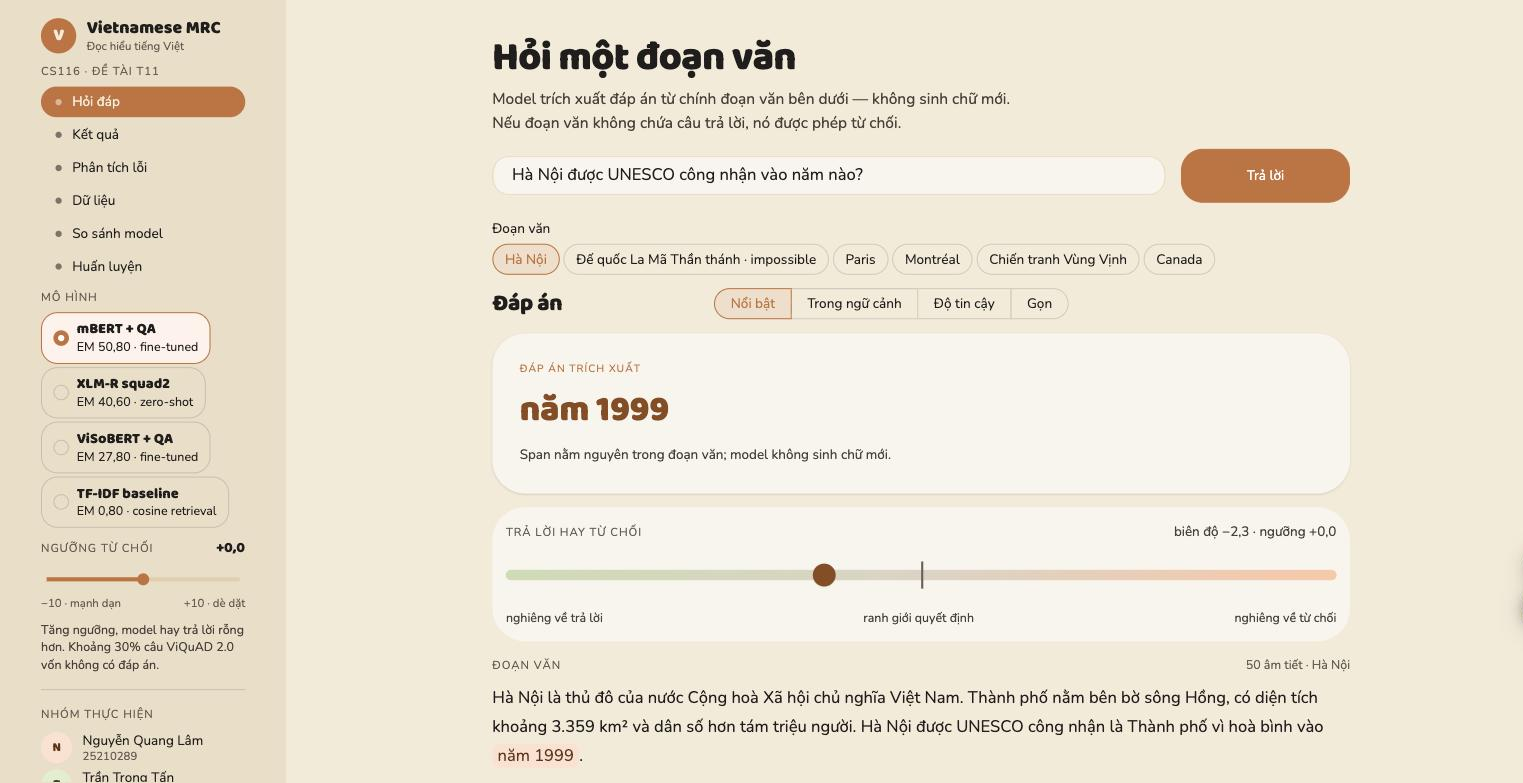
\includegraphics[width=0.96\textwidth]{figures/demo_answerable.png}}
  \caption{Câu hỏi có đáp án ($\tau = 0{,}0$): span được tô sáng trong đoạn văn}
\end{subfigure}\hfill
\begin{subfigure}[t]{0.49\textwidth}
  \centering
  \fbox{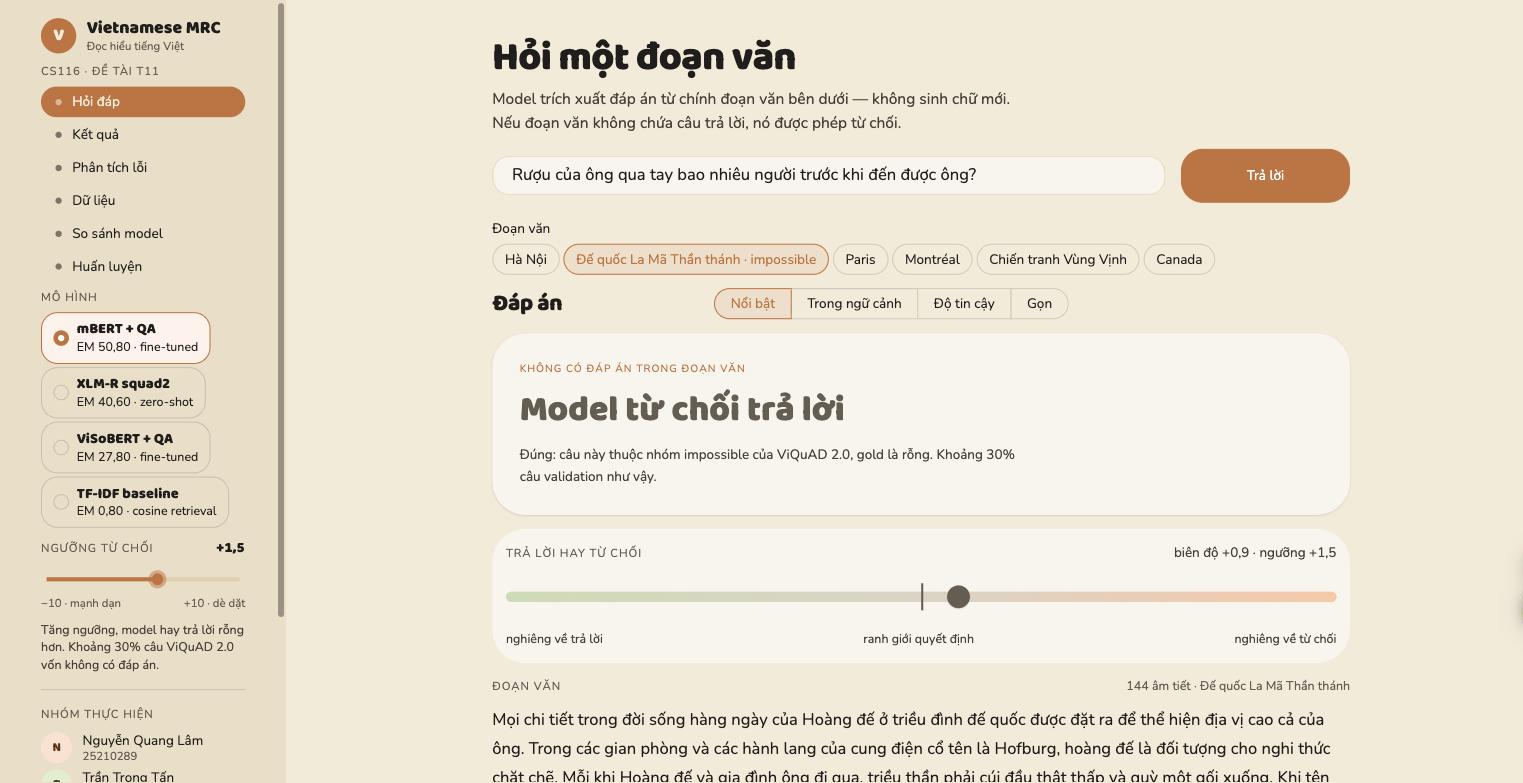
\includegraphics[width=0.96\textwidth]{figures/demo_impossible.png}}
  \caption{Đoạn văn impossible ở $\tau = 1{,}5$: biên độ $+0{,}9$, mô hình từ chối}
\end{subfigure}
\caption{Màn hình Hỏi đáp của ứng dụng web với mô hình mBERT fine-tune. Thanh bên chọn mô hình và ngưỡng $\tau$; thanh ngang dưới thẻ đáp án là biên độ quyết định so với ranh giới}
\label{fig:demo}
\end{figure}
